%iffalse
\let\negmedspace\undefined
\let\negthickspace\undefined
\documentclass[journal,12pt,onecolumn]{IEEEtran}
\usepackage{cite}
\usepackage{amsmath,amssymb,amsfonts,amsthm}
\usepackage{algorithmic}
\usepackage{multicol}
\usepackage{graphicx}
\usepackage{textcomp}
\usepackage{xcolor}
\usepackage{txfonts}
\usepackage{listings}
\usepackage{enumitem}
\usepackage{mathtools}
\usepackage{gensymb}
\usepackage{comment}
\usepackage[breaklinks=true]{hyperref}
\usepackage{tkz-euclide} 
\usepackage{listings}
\usepackage{gvv}                                        
%\def\inputGnumericTable{}                                 
\usepackage[latin1]{inputenc}                                
\usepackage{color}                                            
\usepackage{array}                                            
\usepackage{longtable}                                       
\usepackage{calc}                                             
\usepackage{multirow}                                         
\usepackage{hhline}                                           
\usepackage{ifthen}                                           
\usepackage{lscape}
\usepackage{tabularx}
\usepackage{array}
\usepackage{float}
\newtheorem{theorem}{Theorem}[section]
\newtheorem{problem}{Problem}
\newtheorem{proposition}{Proposition}[section]
\newtheorem{lemma}{Lemma}[section]
\newtheorem{corollary}[theorem]{Corollary}
\newtheorem{example}{Example}[section]
\newtheorem{definition}[problem]{Definition}
\newcommand{\BEQA}{\begin{eqnarray}}
\newcommand{\EEQA}{\end{eqnarray}}
\newcommand{\define}{\stackrel{\triangle}{=}}
\theoremstyle{remark}
\newtheorem{rem}{Remark}

% Marks the beginning of the document
\begin{document}
\bibliographystyle{IEEEtran}
\vspace{3cm}

\title{\textbf{NCERT 9.4.3}}
\author{EE24BTECH11032- John Bobby}
\maketitle
\bigskip
\textbf{Question:} Find the solution for the differential equation $\frac{dy}{dx}+y=1$ using trapezoidal rule.\\
\textbf{Solution:}\\
Let
\begin{align}
    f\brak{x,y}=1-y\\
    y\brak{0}=0
\end{align}
From Forward Euler method:
\begin{align}
\frac{y_{n+1}-y_{n}}{h}=f\brak{x_{n},y_{n}}
\end{align}
From Backward Euler method:
\begin{align}
    \frac{y_{n+1}-y_{n}}{h}=f\brak{x_{n+1},y_{n+1}}
\end{align}
On adding both equation \brak{2} and \brak{3}, We get the Trapezoidal Method
\begin{align}
    \frac{y_{n+1}-y_{n}}{h}=\frac{1}{2}\sbrak{f\brak{x_n,y_n}+f\brak{x_{n+1},y_{n+1}}}\\
    y_{n+1}=y_{n}+\frac{h}{2}\sbrak{f\brak{x_n,y_n}+f\brak{x_{n+1},y_{n+1}}}\\
    y_{n+1}=y_n+\frac{h}{2}\sbrak{1-y_n+1-y_{n+1}}=y_n+\frac{h}{2}\sbrak{2-y_n-y_{n+1}}\\
\end{align}
On rearranging, we get the difference equation
\begin{align}
    y_{n+1}=\frac{2-h}{2+h}y_n+\frac{2h}{2+h}\\ 
    x_{n+1}=x_n +h
\end{align}
\begin{figure}[h!]
    \centering
    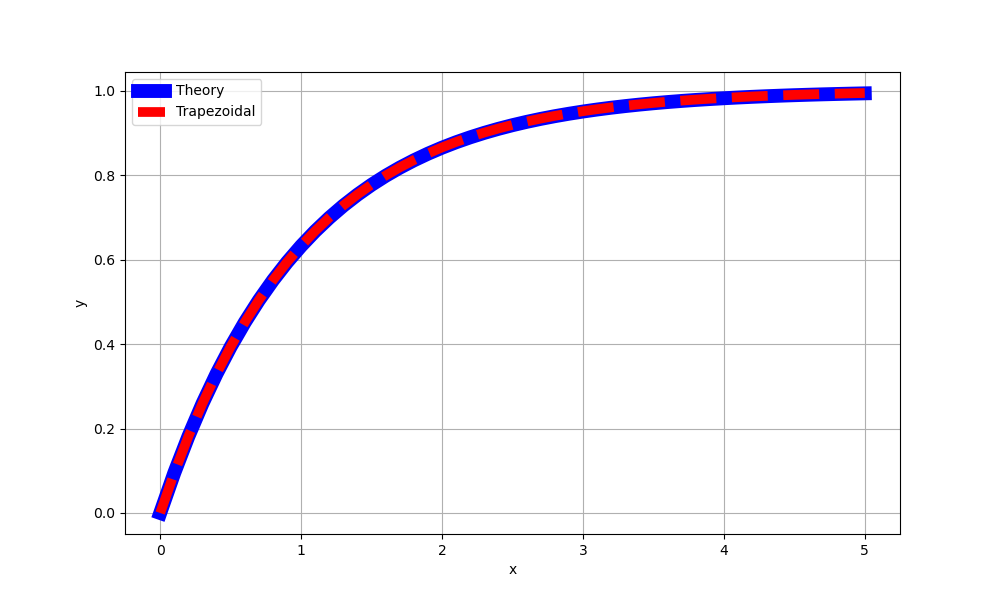
\includegraphics[width=0.7\columnwidth]{figs/Q2.png}
    \label{stemplot}
\end{figure}
\end{document}

